\documentclass[conference]{IEEEtran}

\usepackage{graphicx}
\usepackage{amsmath}
\usepackage{booktabs}
\usepackage{cite}
\usepackage{url}

\title{Characterizing Heterogeneous Edge Inference for Resource-Aware Drone Computing}

\author{
\IEEEauthorblockN{Author Name}
\IEEEauthorblockA{
Department / University\\
Email
}
}

\begin{document}

\maketitle

\begin{abstract}
This work investigates heterogeneous edge inference across Apple Silicon and an Intel/NVIDIA laptop platform as an initial step toward resource-aware scheduling for energy-constrained drone systems. We characterize text and vision workloads of increasing difficulty while varying device, batch size, CPU thread count, numerical precision, and execution backend. Measurements include throughput, latency, accelerator memory usage, power, and energy per processed item. The results show that the best execution configuration depends strongly on workload characteristics and hardware platform. In particular, accelerator choice, CPU parallelism, and numerical precision exhibit distinct performance and resource trade-offs, motivating workload-aware rather than fixed execution policies.
\end{abstract}

\section{Introduction}

Edge AI systems such as autonomous drones operate under strict compute, memory, latency, and energy constraints. Selecting the fastest available accelerator is therefore not always sufficient: an execution configuration must also satisfy resource and endurance requirements.

This work performs an empirical characterization of heterogeneous inference across an Apple M4 platform and an Intel Core i7-11800H system equipped with an NVIDIA RTX 3050 Laptop GPU. Rather than assuming a single optimal device or configuration, we evaluate how workload difficulty, numerical precision, CPU thread count, batch size, and accelerator choice influence inference performance and resource consumption.

The present study provides the characterization foundation for a future resource-aware scheduler. The current contribution focuses strictly on experimentally measured behavior and does not yet claim end-to-end drone endurance improvement or distributed scheduling gains.

\section{Experimental Platforms and Workloads}

\begin{table}[t]
\caption{Experimental Hardware Platforms}
\label{tab:hardware}
\centering
\footnotesize
\resizebox{\columnwidth}{!}{%
\begin{tabular}{llll}
\hline
\textbf{Platform} &
\textbf{CPU} &
\textbf{Accelerator} &
\textbf{Memory Architecture} \\
\hline
Apple M4 system &
Apple M4, 10-core CPU &
Integrated Apple GPU (MPS) &
Unified memory \\
MSI laptop &
Intel Core i7-11800H, 8C/16T &
NVIDIA RTX 3050 Laptop, 4 GB &
System RAM + discrete VRAM \\
\hline
\end{tabular}%
}
\end{table}


We evaluate three text and three vision models representing increasing workload difficulty.

\begin{table}[t]
\caption{Evaluated Workload Matrix}
\label{tab:workloads}
\centering
\footnotesize
\resizebox{\columnwidth}{!}{%
\begin{tabular}{llll}
\hline
\textbf{Modality} &
\textbf{Easy} &
\textbf{Medium} &
\textbf{Hard} \\
\hline
Text &
DistilGPT2 &
Qwen2.5-1.5B &
Qwen3-1.7B \\
Vision &
ResNet50 &
ConvNeXt-Base &
ConvNeXt-Large \\
\hline
\end{tabular}%
}
\end{table}


The text workloads consist of DistilGPT2, Qwen2.5-1.5B, and Qwen3-1.7B. The vision workloads consist of ResNet50, ConvNeXt-Base, and ConvNeXt-Large.

\section{Characterization Methodology}

The characterization study varies execution backend, CPU thread count, batch size, workload intensity, and numerical precision where supported. Short-duration sweeps are used to explore the configuration space, while sustained measurements are used for power and energy characterization.

The primary metrics are inference throughput, latency, accelerator memory allocation, average power, and energy per processed item. Power measurements are interpreted according to their measurement boundary. On Apple M4, the reported value represents combined SoC power, whereas NVIDIA measurements represent GPU board power and Intel CPU measurements represent CPU package power. Consequently, absolute cross-device power and energy values are not treated as directly equivalent measurements.

\section{Results}

\subsection{Cross-Device Throughput}

Figure~\ref{fig:crossover} summarizes the median throughput ratio between matched MSI-side and Apple M4 configurations.

\begin{figure}[t]
    \centering
    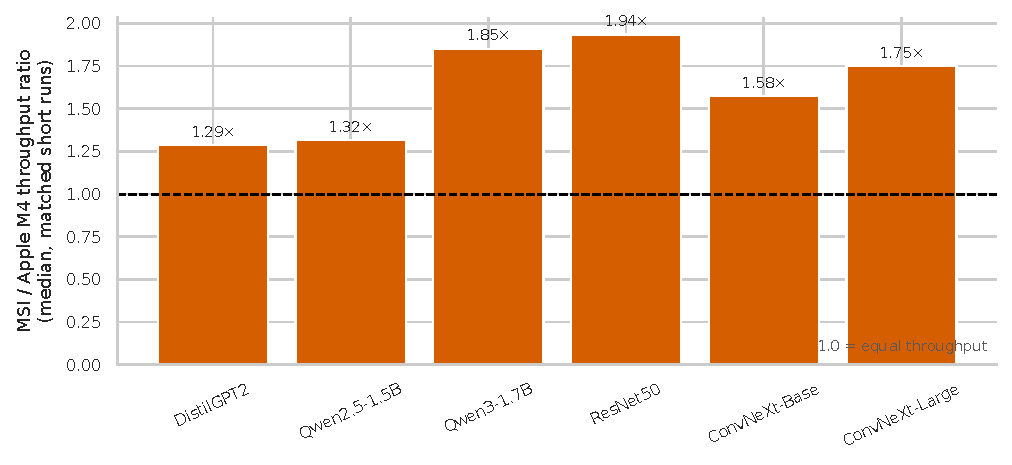
\includegraphics[width=\columnwidth]{figures/fig1_device_crossover.pdf}
    \caption{Median MSI-to-Apple M4 throughput ratio across matched short-run configurations. Values above 1 indicate higher throughput on the MSI-side platform.}
    \label{fig:crossover}
\end{figure}

\begin{table}[t]
\caption{Cross-Device Throughput Summary for Matched Short Runs}
\label{tab:crossover}
\centering
\footnotesize
\resizebox{\columnwidth}{!}{%
\begin{tabular}{llll}
\hline
\textbf{Model} &
\textbf{Modality} &
\textbf{Difficulty} &
\textbf{Median MSI/M4 Ratio} \\
\hline
DistilGPT2 & Text & Easy & 1.29$\times$ \\
Qwen2.5-1.5B & Text & Medium & 1.32$\times$ \\
Qwen3-1.7B & Text & Hard & 1.85$\times$ \\
ResNet50 & Vision & Easy & 1.94$\times$ \\
ConvNeXt-Base & Vision & Medium & 1.58$\times$ \\
ConvNeXt-Large & Vision & Hard & 1.75$\times$ \\
\hline
\end{tabular}%
}
\vspace{1mm}

\scriptsize
A ratio greater than 1 indicates higher throughput on the MSI-side platform for the matched configuration.
\end{table}


The results demonstrate that the relative advantage of the MSI-side platform varies substantially across models, indicating that device selection should depend on workload characteristics rather than a fixed hardware preference.

\subsection{CPU Thread Scaling}

CPU inference does not exhibit a universal optimal thread count.

\begin{figure}[t]
    \centering
    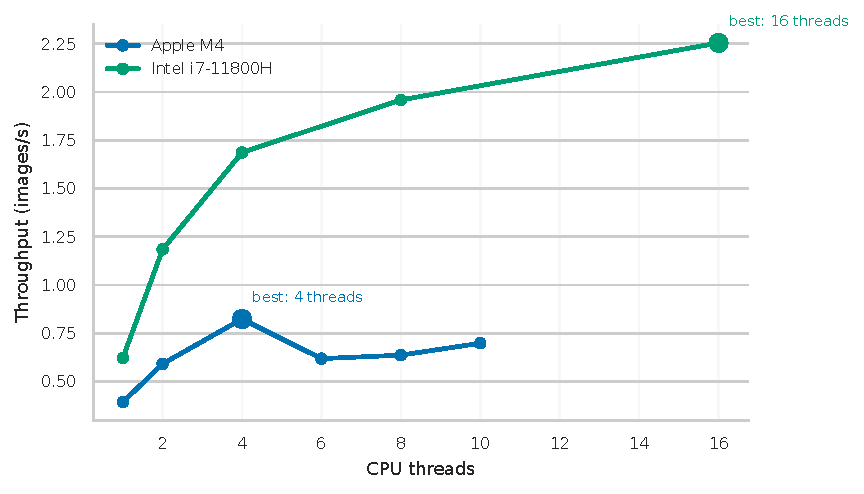
\includegraphics[width=\columnwidth]{figures/fig2_thread_scaling.pdf}
    \caption{CPU thread scaling for ConvNeXt-Large at $320\times320$ resolution and batch size 1. Apple M4 reaches its highest measured throughput at four threads, whereas the Intel i7-11800H continues scaling to sixteen logical threads.}
    \label{fig:threads}
\end{figure}

This behavior suggests that thread-level parallelism must be selected according to the hardware architecture and workload rather than simply maximizing the available thread count.

\subsection{Precision and Throughput}

Numerical precision has a strong impact on accelerator throughput.

\begin{figure}[t]
    \centering
    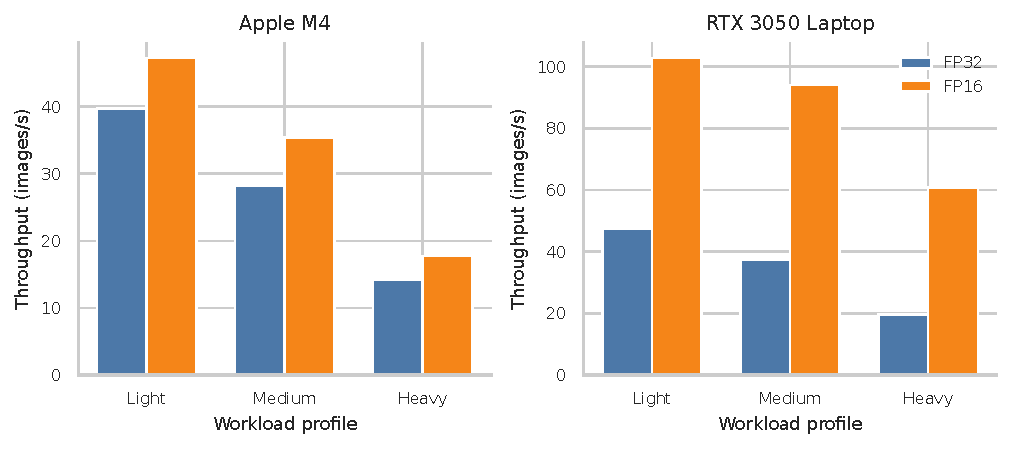
\includegraphics[width=\columnwidth]{figures/fig3_precision_throughput.pdf}
    \caption{Sustained ConvNeXt-Large throughput under FP32 and FP16 execution for representative light, medium, and heavy workloads.}
    \label{fig:precision}
\end{figure}

FP16 improves throughput on both accelerator platforms, with particularly large gains on the RTX 3050 Laptop GPU for medium and heavy configurations.

\subsection{Accelerator Memory Usage}

Precision also affects accelerator memory requirements.

\begin{figure}[t]
    \centering
    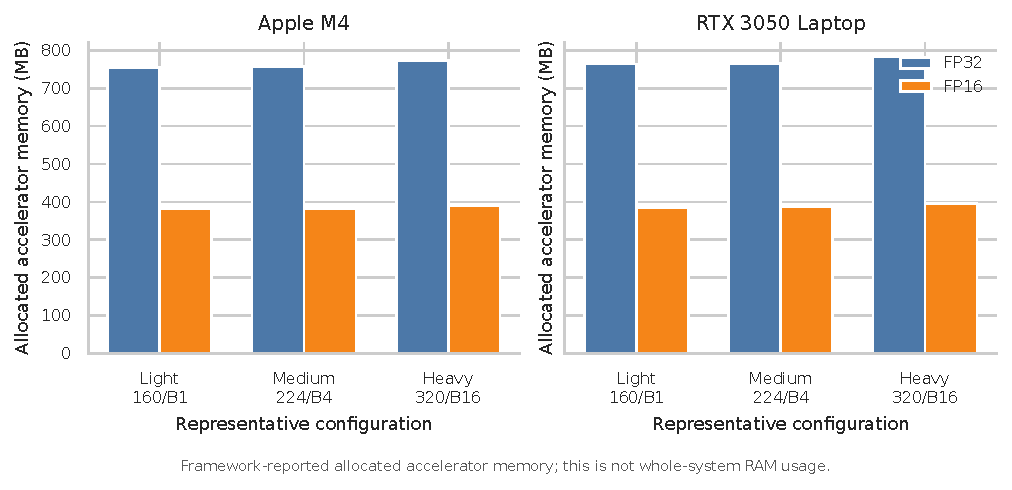
\includegraphics[width=\columnwidth]{figures/fig4_memory_usage.pdf}
    \caption{Framework-reported allocated accelerator memory for representative ConvNeXt-Large configurations. FP16 approximately halves the measured allocation relative to FP32 on both platforms.}
    \label{fig:memory}
\end{figure}

These measurements represent framework-reported accelerator allocation rather than whole-system RAM consumption.

\subsection{Power Characteristics}

\begin{figure}[t]
    \centering
    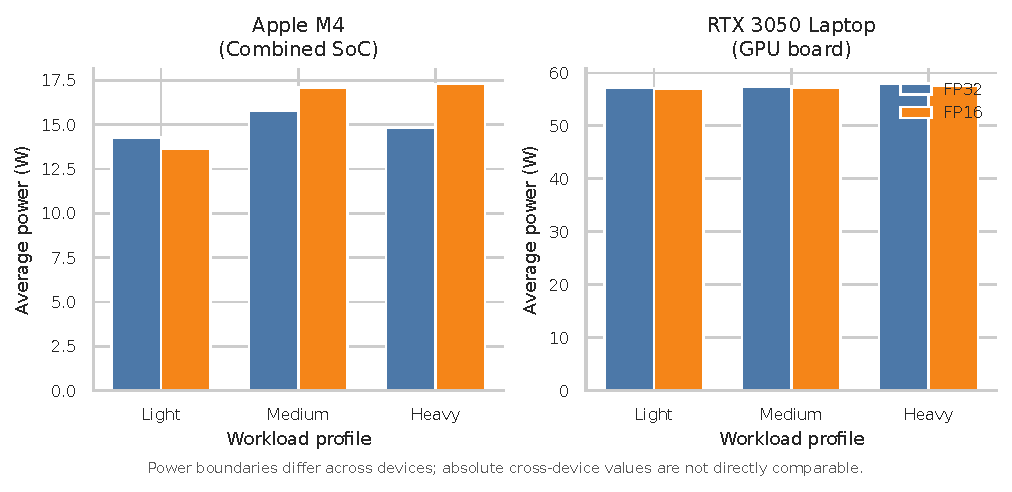
\includegraphics[width=\columnwidth]{figures/fig5_power_consumption.pdf}
    \caption{Sustained average power for ConvNeXt-Large configurations. Apple values represent combined SoC power, while RTX values represent GPU board power; therefore absolute cross-device values are not directly comparable.}
    \label{fig:power}
\end{figure}

The measurements show that throughput improvements do not necessarily correspond to proportional increases in measured power. However, differences in measurement boundaries prevent a direct system-level energy-efficiency ranking between the two platforms.

\subsection{Throughput--Energy Trade-off}

\begin{figure*}[t]
    \centering
    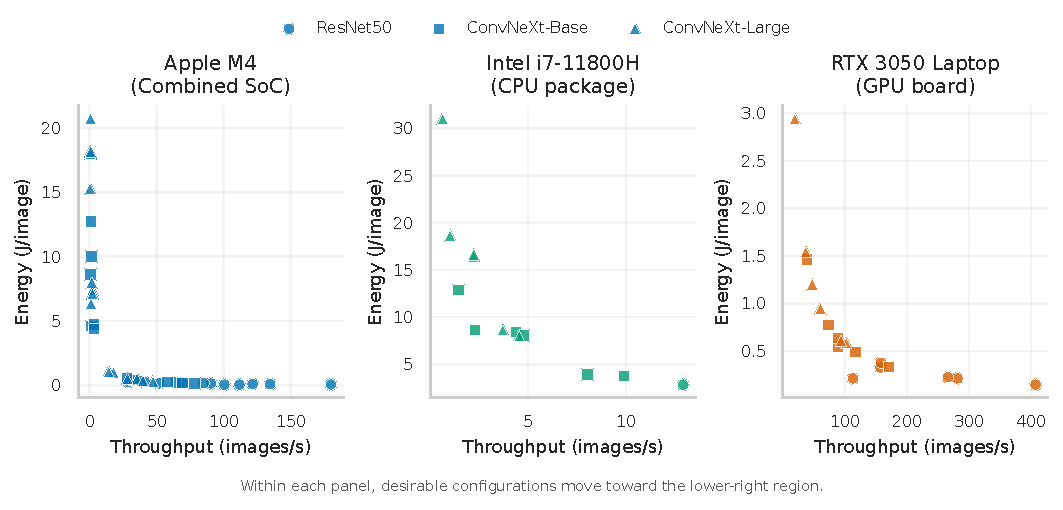
\includegraphics[width=0.95\textwidth]{figures/fig6_speed_energy_tradeoff.pdf}
    \caption{Measured throughput--energy trade-offs for sustained vision workloads. Each panel uses the corresponding device-specific power measurement boundary. Configurations toward the lower-right provide higher throughput at lower measured energy per image within the same panel.}
    \label{fig:energy}
\end{figure*}

The configuration space contains clear throughput--energy trade-offs. In particular, the highest-throughput configuration is not universally the minimum-energy configuration, which provides an empirical motivation for resource-aware execution policies.

\section{Discussion}

The characterization results reveal three important trends. First, device preference changes with workload type and complexity. Second, CPU parallelism exhibits architecture-dependent scaling, meaning that the maximum thread count is not universally optimal. Third, reduced precision can substantially improve throughput and reduce accelerator memory requirements, although its effect on model quality must be evaluated separately.

These observations support the need for a scheduler that considers workload characteristics and resource constraints rather than applying a fixed execution configuration.

\section{Limitations}

The current study characterizes compute resources but does not yet evaluate end-to-end drone battery endurance. Power measurements also use different hardware boundaries across platforms and therefore should not be interpreted as directly comparable whole-system measurements. Model accuracy and task quality under reduced precision have not yet been evaluated. Finally, distributed inference and communication costs are outside the scope of the present characterization stage.

\section{Conclusion}

This study establishes an empirical characterization of heterogeneous edge inference across Apple M4, Intel CPU, and NVIDIA GPU resources. Measurements across six text and vision workloads demonstrate significant variation in throughput, CPU scaling, precision sensitivity, memory demand, power, and energy behavior. These results provide the experimental basis for subsequent resource-aware scheduling research targeting energy-constrained edge systems such as autonomous drones.

\bibliographystyle{IEEEtran}
\bibliography{references}

\end{document}
